\section{O-piccolo}
\definizione{O-piccolo definizione 1}{
Una funzione $ f: A \rightarrow \R$ è \underline{o-piccolo per $x \to x_0$} se esiste una funzione $\omega : A ro \R$ tale che 
\[
f\left( x \right) =g\left( x \right) \omega \left( x \right) \text{ e } \lim_{x \to x_0} \omega =0 
\] 
Si scrive che $f\left( x \right) = o\left( g\left( x \right)  \right) $
}
\definizione{O-piccolo definizione 2}{
Supponiamo di poter dividere per $g\left( x \right) $. Assumiamo quindi $g\left( x \right) \neq 0$ tranne tuttalpiù in $x_0$ allora $f\left( x \right) = o\left( g\left( x \right)  \right) $ se e solo se:
\[
\lim_{x \to x_0} \frac{f\left( x \right) }{g\left( x \right) } =0
\] 
}
\subsection{Proprietà o-piccolo}
\textbf{Somma e differenza di o piccoli}

\[
o\left( g \right) + o\left( g \right)  = o \left( g \right) \quad x \to x_0
\] 
\[
o\left( g \right) - o\left( g \right) = o\left( g \right) \quad x \to x_0
\] 

Dimostrazione:
\vskip3mm
Date due funzioni $f_1\left( x \right)  = o\left( g\left( x \right)  \right) \quad x \to x_0$ e $f_2\left( x \right) = o\left( g\left( x \right)  \right) \quad x \to x_0$
\begin{itemize}
	\item $f_2\left( x \right) = g\left( x \right) \omega_2 \left( x \right) $
	\item $f_1\left( x \right) + f_2\left( x \right) = g\left( x \right) \left( \underbrace{\omega_1\left( x \right) + \omega_2\left( x \right) }_{\omega_3 \to 0} \right) $
\end{itemize}

\textbf{Moltiplicazione per scalare}
\[
k o\left( g \right) = o\left( g \right)  \quad  x \to x_0
\] 

\begin{itemize}
	\item $f_1\left( x \right) = g\left( x \right) \omega_1 \left( x \right) $
	\item $kf_1\left( x \right) = g\left( x \right)\cdot k\omega \left( x \right) = g\left( x \right) \omega \left( x \right)  $
\end{itemize}
\textbf{Prodotto di o-piccoli}
\[
o\left( g \right) o\left( g \right) = o\left( g^2 \right) \quad x \to x_0
\] 
\begin{itemize}
	\item $o\left( g \right) o\left( g \right) = f\left( x \right) f\left( x \right) \omega \left( x \right) \omega \left( x \right)= \left( f\left( x \right) \right) ^2 \omega \left( x \right) ^2 $
	\item $= g^2 \omega \left( x \right) = o\left( g^2 \right)  $
\end{itemize}
\textbf{Transitività o-piccolo}
\begin{gather*}
	f\left( x \right) = o\left( g\left( x \right)  \right) \quad x \to x_0 \\
	g\left( x \right) = o\left( h\left( x \right)  \right) \quad x \to x_0	\\
	\text{ allora }\\
	f\left( x \right) = o\left( h\left( x \right)  \right) \quad x \to x_0
\end{gather*}
\textbf{Prodotto per scalare dell'argomento}
\begin{gather*}
	\text{ se }f\left( x \right) = o\left( g\left( x \right)  \right) \quad x \to 0\\
	\text{ allora }\\
	f\left( kx \right) = o\left( g\left( kx \right)  \right) 
\end{gather*}
\subsection{Sviluppi al primo ordine}
Mentre faccio un limite \underline{per $x \to 0$} posso usare gli sviluppi al primo ordine per rendre tutto molto più semblice:
\begin{align*}
	\sin\left( x \right) &= x + o\left( x \right) & e^{x}&= 1 + x + o\left( x \right) \\
	\cos\left( x \right)&=  1 + o\left( x \right) & \log\left( 1 + x \right) &= x + o\left( x \right) \\
	\cos\left( x \right)  &=  1 + \frac{x^2}{2} + o\left( x^2 \right) & \arctan\left( x \right) &= x + o\left( x \right) \\
	\tan\left( x \right) &=  x + o\left( x \right) & \arcsin \left( x \right) &=  x + o\left( x \right) 
\end{align*}
Posso dimostrarli tutti isolando il $o\left( x \right) $ e facendo il limite per $x \to 0$ di $\frac{f\left( x \right) }{f\left( x \right) }$
\section{Derivate}
\definizione{Derivata con rapporto incrementale}{
In un punto $x_0$ di una funzione la derivata è definita tramite il rapporto incrementale:
\[
	f' \left( x_0 \right) = \lim_{h \to 0} \frac{f\left( x_0 + h \right) - f\left( x_0 \right) }{h} = \lim_{x \to x_0} \frac{f\left( x \right) - f\left( x_0 \right)}{x-x_0}   
\] 
$f\left( x \right) $ è derivabile in $x_0$ se il limite \underline{esiste} ed è \underline{finito}
}
\definizione{Derivata con o piccolo}{
	Dire che esiste la derivata $f' \left( x_0 \right) $ è equivalente a dire che è siddisfatta la seguente relazione:
	\[
		f\left( x_0 + g \right) = f\left( x_0 \right) + f'\left( x_0 \right) h + o\left( h \right) \quad \text{ con } h \to 0	
	\] 
}
Dimostrazione fra le due definzioni:
\begin{itemize}
	\item Supponiamo vera la relazione con l'o piccolo e inseriamola all'interno del rapporto incrementale:
		\[
			f'\left( x_0 \right)  = \frac{f'\left( x_0 +h\right) - f\left( x_0 \right) }{h} = \frac{f'\left( x_0 \right) h + o\left( h \right) }{h} = f'\left( x_0 \right) + \underbrace{\frac{o\left( h \right) }{h}}_{ \to 0 } = f'\left( x_0 \right) 
		\]  
	\item Viceversa: supponiamo vero il limite del rapporto incrementale. Dimostro che 
		\[
			o\left( h \right)  = f\left( x_0 + h \right) - f\left( x_0 \right) - f'\left( x_0 \right) h
		\] 
	\item Calcolo $\lim_{h \to 0} \frac{f\left( h \right) }{g\left( h \right) }$
		\[
			\frac{f\left( x_0+h \right) - f\left( x_0 \right) - f'\left( x_0 \right) h}{h} = \frac{f\left( x_0 +h \right) - f\left( x_0 \right)}{h} - f'\left( x_0 \right) = f'\left( x_0 \right) - f' \left( x_0 \right) =0  
		\] 
\end{itemize}
Quindi le due relazioni sono \underline{reciprocamente implicate}
\subsection{Regole derivazione}
\begin{align*}
	\left( f \pm g \right) ' &= f' \pm g' & \left( \lambda f \right) ' &=  \lambda f'\\
	\left( fg \right) '	&=  f'g + fg' & \left( \frac{f}{g} \right) ' &=  \frac{f'g- g'f}{g^2}\\
	\left( f\left( g\left( x \right)   \right)  \right) '  &=  f'\left( g \right) g'
\end{align*}
\subsubsection{Dimostrazione regole di derivazione}
\[
	\boxed{	\left( fg \right) ' =  f'g + fg'}
\]
\begin{itemize}
	\item Per definizione la derivata è il limite del rapporto incrementale:
		\[
			f'\left( f\left( x \right) g\left( x \right)  \right) = \lim_{h \to 0} \frac{f\left( x_0 +h \right) g\left( x_0+h \right) - f\left( x_0 \right) g\left( x_0 \right) }{h} 
		\] 
	\item Aggiungo e sottraggo $f\left( x_0 +g \right) g\left( o \right) $ 
		\[
			\frac{f\left( x_0+h \right) \underbrace{- f\left( x_0 + h \right) g\left( x_0 \right) + g\left( x_0 + h \right) g\left( x_0 \right)} - f\left( x_0 \right) }{h}
		\] 
	\item Raccolgo primo con secondo e terzo con quarto:
		\[
			f\left( x_0 + h \right) \frac{g\left( x_0 +h \right) - g\left( x_0 \right) }{h} + g\left( x_0 \right) \frac{f\left( x_0 + h \right) - f\left( x_0 \right) }{h}
		\] 
	\item tutto questo è uguale a: 
		\[
			f\left( x_0 \right) g' \left( x_0 \right) + g\left( x_0 \right) f'\left( x_0 \right) 
		\] 
		Questo in quanto $f$ è continua
\end{itemize}
\[
	\boxed{	\left( f\left( g\left( x \right)   \right)  \right) '  =  f'\left( g \right) g'}
\]
\begin{itemize}
	\item 
	i
\end{itemize}
\subsection{Derivate elementari}
\begin{align*}
	&\left( \tan x \right) ' = \frac{1}{\cos ^2 x}=  1 + \left( \tan x \right) ^2 && \left( \arctan  \right) ' =  \frac{1}{1+x^2}\\
	&\left( \arcsin \right) ' =  \frac{1}{\sqrt{1-x^2} }  &&\left( \arccos \right) ' =  -\frac{1}{\sqrt{1-x^2} }\\
	&\left( a^{x} \right) ' =  a^{x} \cdot \log a  
\end{align*}
\subsubsection{Dimostrazione di derivate elemenrari tramite o-piccolo}
\[
	\boxed{	d\left[ e^{x} \right] = e^{x}}
\]
\begin{itemize}
	\item $f\left( x_0 + h \right) = e^{x_0 + h}= e^{x_0 }e ^{ h}$
	\item Applico sviluppi al primo ordine:
		\[
			e^{x_0 }e ^{ h}= e^{x_0}\left( 1+h+ o\left( h \right)  \right) = e^{x}+ e^{x_0}h + e^{x_0}o\left( h \right) 
		\] 
	\item Noto che
		\[
			\underbrace{e^{x}}_{f\left( x_0 \right) }+ \underbrace{e^{x_0}}_{f'\left( x_0 \right) }h + \underbrace{e^{x_0}o\left( h \right)}_{=o\left( h \right) }
		\] 
\end{itemize}
\[
	\boxed{	d\left[ \sin \left( x \right)  \right] }
\]
\begin{itemize}
	\item $f\left( x_0 + h \right) = \sin \left( x_0 + h \right) $
	\item Applico formula somma di seni:
		\[
			\sin \left( x_0 +h \right) = \sin \left( x_0  \right) \cos \left( h \right) + \cos \left( x_0 \right) \sin \left( h \right) 
		\] 
	\item Applico sviluppo al primo ordine di $\sin \left( h \right)$ e $\cos \left( h \right) $
		\[
			\sin \left( x_0 \right) \left( 1+ o\left( h \right)  \right) + \cos \left( x_0 \right) \left( h + o \left( h \right)  \right) 
		\] 
\end{itemize}
\[
	\boxed{	d\left[ \log \left( x_0+h \right)  \right] 
}
\]
\begin{itemize}
	\item $f\left( x_0 + h \right) = \log \left( x_0 +h \right) $
	\item Raccolgo $x_0$ :
		\[
			\log \left( x_0 \left( 1+ \frac{h}{x_0} \right)  \right) 
		\] 
	\item Proprietà dei logaritmi:
		\[
			\log \left( x_0 \right) + \log \left( 1 + \frac{1}{x_0} \right) 
		\] 
	\item Sviluppo al primo ordine di $\log  \left( 1 + \frac{h}{x_0} \right) $ :
		\[
			\log \left( x_0  \right) + \frac{h}{x_0}+ o\left( \frac{h}{x_0} \right) 
		\] 
	\item Per proprietà degli o piccoli $o\left( \frac{h}{x_0} \right) = o\left( h \right) $
	\[
		\underbrace{\log \left( x_0 \right)}_{f\left( x_0 \right) } + \underbrace{\frac{1}{x_0}h}_{f'\left( x_0 \right) } + o\left( h \right) 
	\] 
\end{itemize}
\section{De l'Hopital e Taylor: pilastri della matematica}
\subsection{De l'hopital}
\subsection{Esempi limiti}

\[
	\frac{x - \sin  \left( x \right)  + x^{5}}{x^{3}}
\] 
	 Applico de l'Hopital derivando 3 volte
	 \begin{align*}
		\frac{x - \sin  \left( x \right)  + x^{5}}{x^{3}} &= \\
		&= \lim_{x \to 0} \frac{x - \sin \left( x \right)  + x^{5}}{x^3}   \\
		&= \lim_{x \to 0} \frac{1 - \cos \left( x \right)  + 5x^{4}}{3 x ^2}\\
		&= \lim_{x \to 0} \frac{\sin \left( x \right)  + 20 x^3}{6x} \\
		&=\lim_{x \to 0} \frac{\cos \left( x + 60x^2 \right) }{6} 
	 \end{align*}

\subsection{Taylor}
\teorema{Formula di taylor}{
	Sia $f $ unf funzione e sia $n \in  \N$. Sotto opportune ipotesi esiste un polinomio di grado $\le n, P_n \left( x \right) $ tale che 
	\[
		f\left( x \right) = P_n\left( x \right)  + o\left( x^{n} \right) \quad x \to 0
	\] 
Il polinomio $P_n\left( x \right) $ è dato dalla seguente formulari:
\[
	P_n \left( x \right)  = \frac{f\left( x \right) }{0!} + \frac{f'\left( 0 \right)}{1!}x + \frac{f''\left( 0 \right) }{2!}x^2 + \ldots +  \frac{f^{n}\left( 0 \right) }{n!} x^{n}
\] 
ossia
\[
	\sum_{k=0}^{n} \frac{f^{k}\left( 0 \right) }{k!}x^{k}
\] 
}
\subsubsection{Dimostrazione}
Teorema necessario ai fini della Dimostrazione:
\teorema{}{
Sia $\phi $ una funzione per cui
\[
	\phi \left( 0 \right) = \phi ' \left( 0 \right) + \phi ''\left( 0 \right) +\ldots + \phi ^{n}\left( 0 \right) =0
\] 
Allora
\[
	\phi \left( x \right)  = o \left( x^{n} \right) \quad x \to 0
\] 
}
Dimostrazione:
\begin{itemize}
	\item Applico definizione quasi equivalente per il caso $n=3$ (eivto di fare infinite derivate):
		\[
			\lim_{x \to 0} \frac{\phi \left( x \right) }{x^3} \underbrace{=}_{\text{de l'hopital}} \frac{\phi ' \left( x \right)}{3x^2} = \lim_{x \to 0} \frac{\phi ''' \left( x \right) }{6} = 0  		
		\] 
\end{itemize}
\subsection{Tabella sviluppi di Taylor}
\begin{align*}
	e^{x} &=  1 + x + \frac{x^2}{2!} + \frac{x^{3}}{3!} + \ldots & \log \left( 1+x \right) &= x - \frac{x^2}{2}+ \frac{x^3}{3}- \frac{x^{4}}{4} + \ldots \\ 
	\sin \left( x \right) &=  x - \frac{x^3}{3!} + \frac{x^{5}}{5!}+ \frac{x^{7}}{7!}+ \ldots & \cos \left( x \right) &=  1- \frac{x^2}{2!} + \frac{x^{4}}{4!} - \frac{x^{6}}{6!} \ldots\\
	\sinh \left( x \right) &=  x + \frac{x^3}{3!} + \frac{x^{5}}{5!} + \frac{x^{7}}{7!} \ldots& \cosh \left( x \right) &=  1 + \frac{x^2}{2!} + \frac{x^{4}}{4!} + \frac{x^{6}}{6!} + \ldots \\
	\arctan \left( x \right) &=  x - \frac{x^3}{3} + \frac{x^{5}}{5} - \frac{x^{7}}{7} \ldots & \left( 1+x \right) ^{\alpha }&= 1 + \alpha  x + \frac{\alpha  \left( \alpha  -1 \right) }{2}+ \ldots + \binom{\alpha }{n}x^{n} + \ldots
\end{align*}
\hr
Questi sviluppi si possono dimostrare applicando la definizione e calcolando la derivata, trovando la regola che detta quando questa si annulla

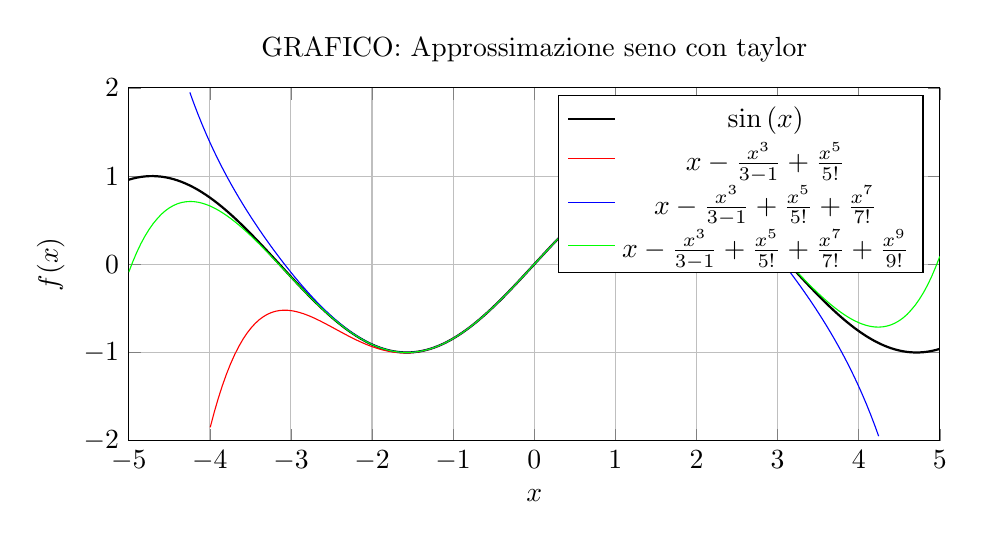
\begin{tikzpicture}
	\begin{axis}[title=GRAFICO: Approssimazione seno con taylor ,
	xmin=-5, xmax=5,
	ymin=-2,ymax=2,
		restrict y to domain = -2:2, domain=-5:5, width=0.98\textwidth, height=0.5\textwidth, grid=major, samples=200,  ylabel=$f(x)$, xlabel=$x$, legend entries={ $\sin \left( x \right) $, $x- \frac{x^3}{3-1} + \frac{x^{5}}{5!}$, $x- \frac{x^3}{3-1} + \frac{x^{5}}{5!} + \frac{x^{7}} {7!}$, $x- \frac{x^3}{3-1} + \frac{x^{5}}{5!} + \frac{x^{7}}{7!}+ \frac{x^{9}}{9!}$}]
		\addplot[black, thick] {sin(deg(x))};
		\addplot[red] {x-(x^3)/6 + (x^5)/5!};
		\addplot[blue] {x-(x^3)/6 + (x^5)/5! - (x^7)/7!};
		\addplot[green] {x-(x^3)/6 + (x^5)/5! - (x^7)/7! + (x^9)/9!};
	\end{axis}
\end{tikzpicture}
\subsection{Sviluppo con Taylor $ \neq 0$}
\label{Taylorno0}
\definizione{Taylor con centro in $x_0$}{
\[
	f\left( x \right) = f\left( x_0 \right) + f'\left( x_0 \right) (x-x_0) + \ldots+ \frac{f^{n}\left( x_0 \right) }{n!}\left( x-x_0 \right) ^{n} + o\left( \left( x-x_0 \right) ^{n} \right) 
\] 
NB: questa formula è equivalente alla formula di Taylor per $ x \to 0$ applicata su una funzione \underline{traslata orizzontalmente verso destra di $x_0$}
}
\incomprensione{10:45:02}
Come cazzo si dimostra?
\begin{itemize}
	\item Calcolando la derivata in $x_0$ ottengo l'approssimazione locale in $ x_0$
	\item Moltiplicando la derivata per $\left( x-x_0 \right) $ traslo il polinomio ottenuto verso destra di $x_0$
\end{itemize}
\section{Teoremi continuoità e derivabilità}
\teorema{Esistenza degli zeri}{
Sia $  f: \left[ a,b \right] \to \R $ una funzione continua. Supponiamo che $  f\left( a \right)  \cdot f\left( b \right)  < 0 $ (ossia che che $ a $ e $ b $ hanno segno discorde). Allora
\[
\exists c \in  \left( a,b \right) \text{ t.c. } f\left( c  \right) =0
\] 
}
NB: posso applicare una variante del teorema. Se $ f : \left[ a,b \right] \to \R $ è continua e $ f\left( a \right) < \lambda  $ e $ f\left( b \right) > \lambda  $ o viceversa, allora
\[
\exists x_0  \text{ t.c. } f\left( x_0 \right) = \lambda 
\] 
Posso generalizzare ulteriormente tramite il teorema dei valori intermedi:
\teorema{Teorema dei valore intermedi}{
Sia $  f: \left( a,b \right) \to \R $ una funzione continua. Sia \[
L = sup \left\{ f\left( x \right) : x \in  \left( a,b \right)  \right\} \text{ e } l = \infty\left\{ f\left( x \right) : x \in  \left( a,b \right)  \right\} 
\] 
Sia $ \lambda   \in  \R$ tale che $ l < \lambda  < L $. Allora 
\[
\exists c \in  \left( a,b \right) \text{ t.c. } f\left( c \right) = \lambda 
\] 
}
Questo equivale a dire che una funzione continua in un intervallo $ \left[ a,b \right]  $ assume tutti i valori compresi fra il suo massimo e il suo minimo. NB: da questo teorema posso ricavare il fatto generale che se:
\[
\lim_{x \to \infty} f(x) = + \infty \text{ e } \lim_{x \to -\infty} f(x) = -\infty
\] 
oppure viceversa, allora $ f\left( x \right)  $ è surgettiva
\subsection{Teoremi studio locale funzione}
\teorema{Criterio di monotonia 1}{
Sia $  f: A \to \R  $ e $ x_0 \in  A $. Supponiamo che $ f'\left( x \right) > 0 $. Allora esiste $ \delta >0 $ tale che:
\begin{itemize}
	\item $ f\left( x \right)  > f\left( x_0 \right) \quad  \forall x \in  \left( x_0 , x_0+ \delta   \right)  $
	\item $ f\left( x \right)  < f\left( x_0 \right) \quad  \forall x \in  \left( x_0- \delta , x_0  \right)  $
\end{itemize}
}
NB: l'affermazione si limita allo studio \underline{locale} di una funzione. La funzione è quindi \underline{crescente} ma \underline{solo localmente}
\definizione{Punto stazionario}{
Sia $ f $ derivabile in $ x_0 $. Se $ f'\left( x_0 \right)  $ allora il punto $ x_0 $ è detto \underline{ punto stazionario}
}
NB: ho 5 possibili punti stazionari:
	\begin{itemize}
		\item Punto di massimo
		\item Punto di minimo
		\item Flesso a tangenza orizzontale ascendente
		\item Flesso a tangenza orizzontale discendente
		\item Funzioni patologiche che oscillano in a fucked-up fashion
	\end{itemize}
Esempio di quest'ultimo caso:
\[
f\left( x \right)  =
\begin{cases}
	x^2 \sin \left( \frac{1}{x} \right) \quad x \neq 0	\\
	0 \quad x=0
\end{cases}
\] 
\begin{center}
	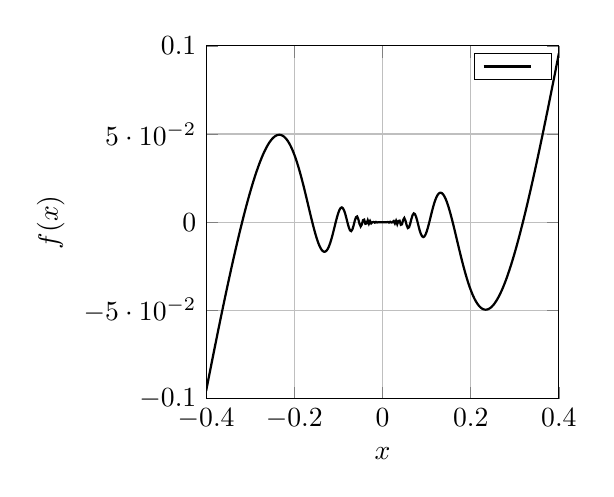
\begin{tikzpicture}
		\begin{axis}[
		xmin=-0.4, xmax=0.4,
		ymin=-0.1,ymax=0.1,
		restrict y to domain = -0.1:0.1, domain=-0.4:0.4, width=0.5\textwidth, height=0.5\textwidth, grid=major, samples=300,  ylabel=$f(x)$, xlabel=$x$, legend entries={$ $}]
		\addplot[black, thick] {x^2*sin(deg(1/x))};
		\end{axis}
	\end{tikzpicture}
\end{center}
Questa funzione oscilla sempre più avvicinandosi all'origine, ma la derivate in 0 esiste ed è nulla
\teorema{Criterio delle derivate successive}{
Immagino di cercare la prima derivata che non si annulla in un punto $ x_0 $. Supponiamo che questa derivata sia di ordine $ k $:
\[
f'\left( x_0 \right) =f''\left( x_0 \right) =f'''\left( x_0 \right)=f^{\left( k-1 \right) }\left( x_0 \right)  =0 
\]
ho 4 opzioni:

\begin{center}
	\begin{forest}
	[k, for tree={forked edges, draw=gray!20, align=left, grow'=0}
		[ è pari 
			[ $ f^{k}(x_0) > 0 $
				[$x_0$ è \underline{minimo locale}]
			]
			[ $ f^{k}(x_0) < 0 $
				[$x_0$ è \underline{minimo locale}]
			]
		]
		[ è dispari 
			[ $ f^{k}(x_0) > 0 $
				[$x_0$ è flesso a tg. orizzontale \underline{ascendente}]
			]
			[ $ f^{k}(x_0) < 0 $
				[$x_0$ è flesso a tg. orizzontale \underline{discendente}]
			]
		]
	]
\end{forest}
\end{center}
}
Dimostrazione: la dimostrazione è interesante e usa lo sviluppo di Taylor
\begin{itemize}
	\item Calcolo sviluppo di Taylor in $  x_0 $ in modo tale da approssimare concavità della funzione (vedi \textit{sezione \ref{Taylorno0}})
	\[
	f\left( x \right) = f\left( x_0 \right)  + f'\left( x_0 \right) \left( x-x_0 \right) +\ldots+ \frac{f^{k}\left( x_0 \right)}{k!}\left( x-x_0 \right) ^{k} + o\left( \left( x-x_0 \right) ^{k} \right)  \quad \text{ per } x \to x_0
	\] 
	\item Per un valore di $ h $ molto piccolo posso calcolare il polinomio in $ x_0+h $, visto che non mi distaccherei troppo dall'intorno in cui il polinomio è approssimato bene:
	\[
	f\left( x_0+h \right) = f\left( x_0 \right) + f'\left( x_0 \right) h + \ldots + \frac{f^{k}\left( x_0 \right)}{k!}h^{k} + o \left( h^{k} \right)  
	\] 
	\item Noto che per ipotesi le derivate di ordine $ 1,\ldots,k-1 $ sono tutte nulle, quindi lo sviluppo di Taylor è il seguente:
	\[
	f\left( x_0+h \right) = \frac{f^{k}\left( x_0 \right)}{k!}h^{k}+ o\left( h^{k} \right)  
	\] 
	\item Dividendo per $ h^{k} $ elimino l'o-piccolo per definizione e ottengo:
	\[
	\frac{f\left( x_0+h \right)- f\left( x_0 \right) }{h^{k}}= \frac{f^{\left( k \right) }\left( x_0 \right) }{k!}
	\] 
	\item Noto che ho a destra la derivata \textit{k-esima} di $ f $. Riprendendo le affermazioni riguardo segno della derivata e parità di $ k $ posso osservare che, ad esempio, se $ f\left( x_0 +h\right)  > f\left( x_0 \right) $ $ x_0 $ è un punto di minimo locale. Le stesse affermazioni si possono fare per i flessi e i massimi
	\end{itemize}

\teorema{Teorema di Weierstrass}{
Sia $f : \left[ a,b \right] $ una funzione continua nell'intervallo $\left[ a,b \right] $. Allora esistono almeno un massimo e un minimo assoluto in $\left[ a,b \right] $
}
Varianti Weierstrass:
\begin{itemize}
	\item Sia $  f: \R \to \R $ continua e \underline{periodica}. Allora esistono MAX e MIN
	\item Sia $  f: \R \to \R $ continua. Supponiamo che 
	\[
	\lim_{x \to +\infty} f(x) = \lim_{x \to -\infty} f(x) = \pm \infty
	\] 
	allora esiste MIN/MAX (rispettivamente per $ +\infty/-\infty $)
\end{itemize}

\teorema{Teorema di Rolle}{
Sian $f: \left[ a,b \right]  \to \R$. Supponiamo che 
\begin{itemize}
	\item $f$ è continua in $\left[ a,b \right] $
	\item $f$ è derivabile in $ \left( a,b \right) $
	\item $f\left( a \right) = f\left( b \right) $
\end{itemize}
allora 
\[
\exists x_0 \in  \left( a,b \right) \text{ t.c. } f'\left( x_0 \right) =0
\] 
}
\teorema{Teorema di Cauchy}{
Siano $f:\left[ a,b \right] \to \R, \quad  g:\left[ a,b \right] \to \R$. Supponiamo che 
\begin{itemize}
	\item $f$ e $g$ sono continue in $\left[ a,b \right] $
	\item $f$ e $g$ sono derivabili in $ \left( a,b \right) $
\end{itemize}
Allora $\exists x_0 \in  \left( a,b \right)$  tale che 
\[
\left( f\left( b \right) - f\left( a \right)  \right) g'\left( x_0 \right) = \left( g\left( x \right) -g\left( a \right)  \right) f_0\left( x_0 \right) 
\] 
se inoltre 
\begin{itemize}
	\item  $g'\left( x \right) \neq 0 \quad \forall x \in \left( a,b \right) $
\end{itemize}
allora $g\left( b \right) \neq g\left( a \right) $ e dividendo per $g_0\left( x_0 \right) $ ottengo
\[
\frac{f\left( b \right) - f\left( a \right) }{g\left( b \right) -g\left( a \right) }= \frac{f'\left( x_0 \right)}{g'\left( x_0 \right) } 
\] 
}
NB: se penso a teorema di Lagrange, noto che il rapporto fra le derivate è esattamente il rapporto fra i $ \Delta  y$ che la funzione assume agli estremi:
\[
f'\left( x_0 \right) = \frac{f\left( b \right) -f\left( a \right)}{b-a} \quad g'\left( x_0 \right) = \frac{g\left( b \right) - g\left( a \right) }{b-a}
\] 
Facendo il rapporto $  b-a $ si annulla e ottengo esattamente quanto espresso da teorema di Cauchy
\vskip3mm
Dimostrazione:
\begin{itemize}
	\item Uso rolle su una nuova funzione definita nel seguente modo:
	\[
	\phi \left( x \right) = \left( f\left( b \right) -f\left( a \right)  \right) g\left( x \right) - \left( g\left( b \right) -g\left( a \right)  \right) f\left( x \right) 
	\] 
	\item Noto che 
	\begin{itemize}
		\item $\phi $ è continua in $\left[ a,b \right] $ in quanto \textit{combinazione lineare }di funzioni derivabili
		\item $\phi $ è derivabile in $ \left( a,b \right) $ in quanto \textit{combinazione lineare }di funzioni derivabili
		\item $\phi\left( a \right) = \phi \left( b \right)  $. Basta verificare inserendo $a$ e $b$
	\end{itemize}
\item La funzione soddisma le ipotesi del \underline{teorema di Rolle} ossia:
\[
	\phi' \left( x \right) = \left( f\left( b \right) -f\left( a \right)  \right) g'\left( x \right) - \left( g\left( b \right) -g\left( a \right)  \right) f'\left( x \right) =0
\] 
ottengo quindi l'ipotesi 1 del teorema
\end{itemize}
\teorema{Teorema di Lagrange}{
Sia $f:\left[ a,b \right] \to \R$. Supponiamo che 
\begin{itemize}
	\item f è continua in  $\left[ a,b \right] $
	\item f è derivabile in $\left( a,b \right) $
\end{itemize}
Allora $\exists x_0 \in  \left( a,b \right) \text{ t.c. }$ 
\[
f\left( b \right) - f\left( a \right) = f'\left( x_0 \right) \left( b-a \right) 
\] 
}
Dimostrazione:
\begin{itemize}
	\item Uso teorema di Cauchy con $g\left( x \right) =x$
	\[
	\frac{f\left( b \right) -f\left( a \right) }{b-a}=f'\left( x_0 \right) 
	\] 
\end{itemize}
\teorema{Teorema monotonia 2}{
Sia $f:\left[ a,b \right] \to \R$. Supponiamo
\begin{itemize}
	\item $f$ continuo in $\left[ a,b \right] $
	\item $f$ derivabile in $\left( a,b \right) $
\end{itemize}
allora
\begin{itemize}
	\item Se $ f'\left( x \right) > 0 \quad \forall x \in  \left( a,b \right) \Rightarrow f$ è strettamente crescente
	\item Se $f'\left( x \right) \ge 0 \quad \forall x \in  \left( a,b \right) \Rightarrow f$ è debolmente crescente
	\item Se $f$ è strettamente crescente allora $ f_0\left( x \right)  \ge 0 \quad  \forall x \in  \left( a,b \right) $
	\item Se $f$ è debolmente crescente allora $ f_0\left( x \right) \ge 0 \quad \forall x \in  \left( a,b \right) $
\end{itemize}
}
Dimostrazione:
\begin{itemize}
	\item Per ipotesi $f$ è debolmente crescente. Prendo $x_0 \in  \left( a,b \right) $ 
	\[
	f'\left( x_0 \right) = \lim_{h \to 0^{+}} \frac{f\left( x_0+h \right) -f\left( x_0 \right)}{h}  
	\] 
	\item Se $f$ è crescente allora il denominatore del rapporto incrementale è \underline{positivo}. Il limite per $h \to o^{+}$ è quindi positivo.
\end{itemize}
\hr
\begin{itemize}
	\item Per ipotesi $f_0\left( x \right) > 0 \quad  \forall x \in  \left( a,b \right) $
	\item Applico Lagrande a $\left[ c,d \right] \subseteq \left[ a,b \right] $ e ottengo:
	\[
	f\left( d \right) - f\left( c \right) =f'\left( x_0 \right) \left( d-c \right) 
	\] 
	\item Siccome $f'\left( x \right) > 0$ per ipotesi e $\left( d-c \right) > 0$ allora $f\left( d \right) -f\left( c \right) > 0$
	\item Vista l'arbitrarietà nella scelta di $d$ e $c$ posso affermare che $f$ è crescente
\end{itemize}
\teorema{Teorema monotonia 3}{
Sia $f:\left[ a,b \right] \to \R$. Supponiamo che 
\begin{itemize}
	\item $f$ è continua in $\left[ a,b \right] $
	\item $f$ è derivabile in $ \left( a,b \right) $
	\item $f'\left( x \right)  \ge 0 \quad \forall x \in  \left( a,b \right) $
	\item Non esiste alcun intervallo contenuto in $\left( a,b \right) $ in cui $f'$ è sempre $=0$. E' possibile tuttavia che $f'\left( x \right) =0$ in punti isolati (\textit{sporadicamente})
\end{itemize}
allora
\[
f \text{ è strettamente crescente in } \left( a,b \right) 
\] 
}
Dimostrazione:
\begin{itemize}
	\item Per ipotesi $f$ è debolmente crescente: se non fosse strettamente crescente vorrebbe dire che c'è un intervallo in cui $f$ è costante. Questo però viola la condizione 4 per cui $f$ è strettamente crescente
\end{itemize}
\definizione{Lipschizzianità}{
Sia $ A \in  \R$ e sia $ f: A \to \R$. si dice che $f$ è lipschizziana in $A$ se esiste $L \in  \R$ tale che $ \forall x, y \in  A$ si ha
\[
	\left|f\left( x \right)  - f\left( y \right) \right| \le L \left| x-y\right|
\] 
}
Esempi:

\begin{minipage}[t]{0.48\textwidth}
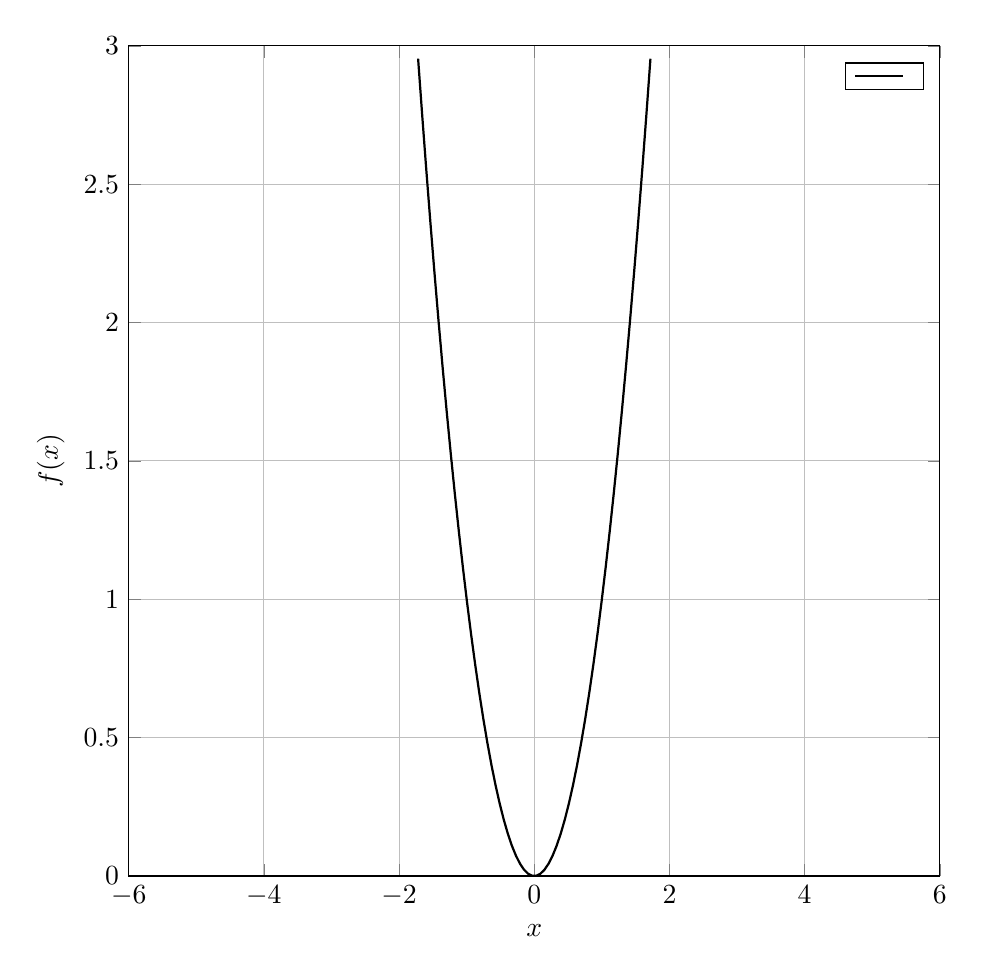
\begin{tikzpicture}
	\begin{axis}[xmin=-6, xmax=6,
	ymin=0,ymax=3,
	restrict y to domain = 0:3, domain=-6:6, width=0.98\textwidth, height=\textwidth, grid=major, samples=200,  ylabel=$f(x)$, xlabel=$x$, legend entries={$ $}]
	\addplot[black, thick] {x^2};
	\end{axis}
\end{tikzpicture}
	No, se $x \to \infty$ la pendenza è infinita. Sì se considero intervallo $\left[ -1,1 \right] $
\end{minipage}
%
\begin{minipage}[t]{0.48\textwidth}
\begin{tikzpicture}
	\begin{axis}[xmin=-6, xmax=6,
	ymin=0,ymax=8,
	restrict y to domain = 0:3, domain=-6:6, width=0.98\textwidth, height=\textwidth, grid=major, samples=200,  ylabel=$f(x)$, xlabel=$x$, legend entries={$ $}]
		\addplot[black, thick] {sqrt(x)};
	\end{axis}
\end{tikzpicture}
	No, se $x \to 0$ la pensenza è infinita. Si se considero intervallo $[1, + \infty)$
\end{minipage}
\teorema{Continuità e lipschizianità}{
Sia $ f A \to \R$ lipschizziana. Allora
\[
f \text{ continua in } A
\] 
}
\teorema{Continuità e lipschizianità 2}{
Sia  $ F: A \to \R$ con $A$ \underline{convesso}. Allora 
\[
	f \text{ è lipschizziana in }A \Leftrightarrow \left|f'\left( x \right) \right| \text{ è limitato }
\] 
in più, in quest'ultimo caso si ha che 
\[
	L = sup\left( \left|f'\left( x \right) \right| : x \in  \left[ 0,1 \right]   \right) 
\] 
}
NB: 
\textbox{
Posso sfruttare quest'ultimo teorema per ottenere importanti disuguaglianze. 
}
Se trovo la minima costante di lipschiz posso applicare la definizione per ottenere la disuguaglianza

